%Galera_counter_example_delete.tex



\begin{figure}[c]{0.5\textwidth}
 %   \centering
    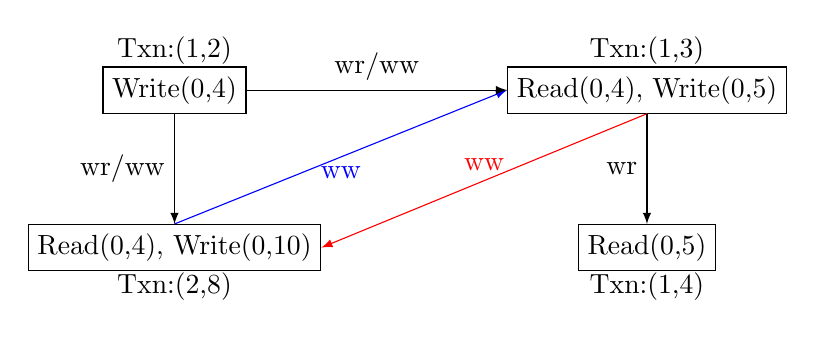
\begin{tikzpicture}[model/.style = {draw, minimum size = 15pt},  node distance = 0.5cm and 1.5cm]
        \node[model] (13) at (6,2) {Read(0,4), Write(0,5)};
        \node (textof13) at (6,2.5) {Txn:(1,3)};
        \node[model] (28) at (0,0) {Read(0,4), Write(0,10)};
        \node (textof28) at (0,-0.5) {Txn:(2,8)};
        \node[model] (14) at (6,0) {Read(0,5)};
        \node (textof14) at (6,-0.5) {Txn:(1,4)};
        \node[model] (12) at (0,2) {Write(0,4)};
        \node (textof12) at (0,2.5) {Txn:(1,2)};
        \path[-latex, color=red] (13.south) edge node[above] {ww} (28.east); 
        \path[-latex, color=blue] (28.north) edge node[below] {ww} (13.west); 
        \path[-latex] (12.east) edge node[above] {wr/ww} (13.west);
        \path[-latex] (12.south) edge node[left] {wr/ww} (28.north);
        \path[-latex] (13.south) edge node[left] {wr} (14.north);
    \end{tikzpicture}
    \caption{Delete uncertainty.}
    \label{fig:delete-galera}
\end{figure}